\begin{figure*}[tp]

\centering

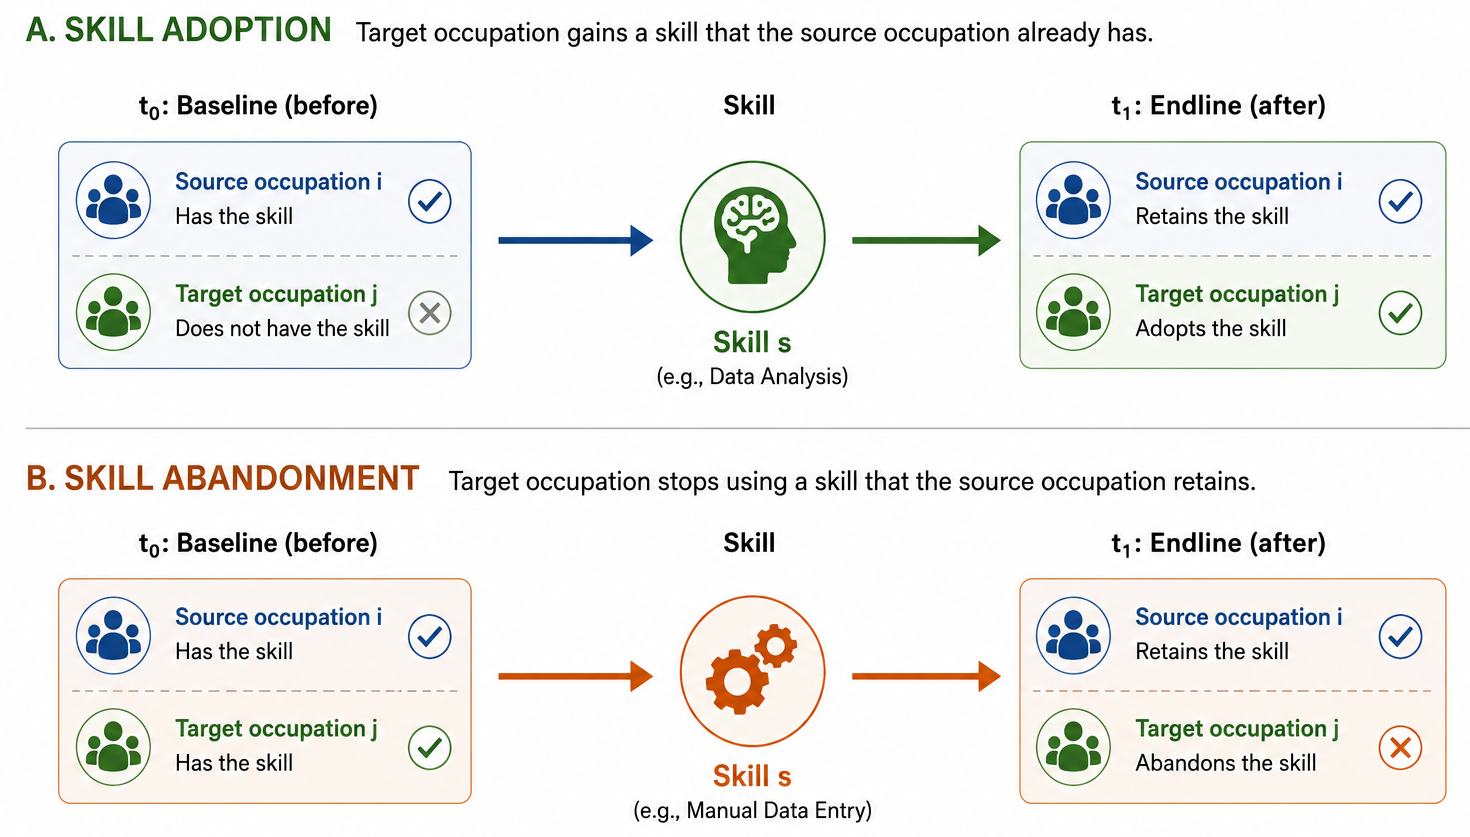
\includegraphics[width=.88\textwidth]{figures/illustration.png}

\caption{\textbf{The two elementary events the analysis is built from.} In an \emph{adoption} event, a target occupation $j$ that lacks a skill comes to hold it under positional pressure from source occupations $i$ that already do; in an \emph{abandonment} event, $j$ sheds a skill that source occupations $i$ retain. The analysis aggregates millions of such directed dyads to ask, for each event, not merely whether a skill moves but on which side of the status gap it lands. We do not observe transmission along particular dyads; we observe that an occupation's likelihood of gaining or losing a requirement moves with the status configuration of all the occupations that hold it.}

\label{fig:diffusion-schematic}

\end{figure*}
